\documentclass[11pt, letterpaper]{article}

\usepackage{multirow}
\usepackage{array}
\usepackage{booktabs}
\usepackage{graphicx}
\usepackage{floatrow}
\usepackage{longtable}
\usepackage{changepage}

\graphicspath{{/}}


\title{HTML and CSS}
\date{2015-10-30}
\author{Creativity Through Code}

\begin{document}
	\maketitle
	\newpage
	\begin{abstract}
		After the introducing the essentials of web development, we will be learning how we can create a beautiful static website using HTML and CSS.
	\end{abstract}
	\section{HTML}
		\textbf{HyperText Markup Language (HTML)} is the standard markup language used to created webpages. It is the building blocks of all websites and it provides the means to create structured documents by denoting structural semantics for text.
		\begin{longtable}{l p{10cm} l}
			\toprule
			Tag & Description \\\midrule
			\texttt{<!---...--->} & Defines a comment \\\midrule
			\texttt{<!DOCTYPE>} & Defines the document type \\\midrule
			\texttt{<a>} & Defines a hyperlink \\\midrule
			\texttt{<abbr>} & Defines an abbreviation or an acronym \\\midrule
			\texttt{<address>} & Defines contact information for the author/owner of a document \\\midrule
			\texttt{<area>} & Defines an area inside an image­map
\\\midrule
			\texttt{<b>} & Defines bold text \\\midrule
			\texttt{<base>} & Specifies the base URL/target for all relative URLs in a document \\\midrule
			\texttt{<bdo>} & Overrides the current text direction \\\midrule
			\texttt{<blockquote>} & Defines a section that is quoted from another source \\\midrule
			\texttt{<body>} & Defines the document's body \\\midrule
			\texttt{<br>} & Defines a single link break \\\midrule
			\texttt{<button>} & Defines a clickable button \\\midrule
			\texttt{<caption>} & Defines a table caption \\\midrule
			\texttt{<cite>} & Defines the title of a work\\\midrule
			\texttt{<code>} & Defines a piece of computer code\\\midrule
			\texttt{<col>} & Specifies column properties for each column within a \texttt{<colgroup>} element\\\midrule
			\texttt{<colgroup>} & Specifies a group of one or more columns in a table for formatting\\\midrule
			\texttt{<dd>} & Defines a description/value of a term in a dsecription list\\\midrule
			\texttt{<del>} & Defines text that has been deleted from a document\\\midrule
			\texttt{<dfn>} & Represents the defining instance of a term \\\midrule
			\texttt{<div>} & Defines a section of a document\\\midrule
			\texttt{<dl>} & Defines a description list\\\midrule
			\texttt{<dt>} & Defines a term/name in a description list\\\midrule
			\texttt{<em>} & Defines emphasized text \\\midrule
			\texttt{<fieldset>} & Groups related elements in a form\\\midrule
			\texttt{<footer>} & Defines a footer for a document or section\\\midrule
			\texttt{<form>} & Defines a HTML form for user input\\\midrule
			\texttt{<h1> to <h6>} & Defines HTML headings\\\midrule
			\texttt{<head>} & Defines information about the document\\\midrule
			\texttt{<header>} & Defines a header for a document or section\\\midrule
			\texttt{<hr>} & Defines a thematic change in the content\\\midrule
			\texttt{<html>} & Defines the root of an HTML document\\\midrule
			\texttt{<i>} & Defines a part of text in italics\\\midrule
			\texttt{<iframe>} & Defines an inline frame\\\midrule
			\texttt{<img>} & Defines an image\\\midrule
			\texttt{<input>} & Defines an input control\\\midrule
			\texttt{<ins>} & Defines a text that has been inserted into a document\\\midrule
			\texttt{<kbd>} & Defines keyboard input\\\midrule
			\texttt{<labe>} & Defines a label for an \texttt{<input>} element\\\midrule
			\texttt{<legend>} & Defines a cptaion for a \texttt{<fieldset>} element\\\midrule
			\texttt{<li>} & Defines a list item\\\midrule
			\texttt{<link>} & Defines relationship between document and external resource\\\midrule
			\texttt{<map>} & Defines a client-side image-map\\\midrule
			\texttt{<menu>} & Defines a list/menu of commands\\\midrule
			\texttt{<menuitem>} & Defines a menu/command item\\\midrule
			\texttt{<meta>} & Defines metadata about an HTML document\\\midrule
			\texttt{<meter>} & Defines a scalar measurement within a known range\\\midrule
			\texttt{<nav>} & Defines navigation links\\\midrule
			\texttt{<noscript>} & Defines an alternate content for users\\\midrule
			\texttt{<object>} & Defines an embedded object\\\midrule
			\texttt{<ol>} & Defines an ordered list\\\midrule
			\texttt{<optgroup>} & Defines a group of related option in a drop-down list\\\midrule
			\texttt{<option>} & Defines an option in a drop-down list\\\midrule
			\texttt{<p>} & Defines a paragraph\\\midrule
			\texttt{<param>} & Defines a parameter for an object\\\midrule
			\texttt{<pre>} & Defines preformatted text\\\midrule
			\texttt{<q>} & Defines a short quotation\\\midrule
			\texttt{<s>} & Defines text that is no longer correct\\\midrule
			\texttt{<samp>} & Defines sample output from a computer program\\\midrule
			\texttt{<script>} & Defines a client-side script\\\midrule
			\texttt{<select>} & Defines a drop-down list\\\midrule
			\texttt{<small>} & Defines smaller text\\\midrule
			\texttt{<span>} & Defines a section in a document\\\midrule
			\texttt{<strong>} & Defines important text\\\midrule
			\texttt{<stlye>} & Defines style information for a document\\\midrule
			\texttt{<sub>} & Defines subscripted text\\\midrule
			\texttt{<sup>} & Defines superscripted text\\\midrule
			\texttt{<table>} & Defines a table\\\midrule
			\texttt{<tbody>} & Groups a body content in a table\\\midrule
			\texttt{<td>} & Defines a cell in a table\\\midrule
			\texttt{<textarea>} & Defines a multiline input control\\\midrule
			\texttt{<tfoot>} & Groups the footer content in table\\\midrule
			\texttt{<th>} & Defines a header cell in a table\\\midrule
			\texttt{<thead>} & Groups the header content in a table\\\midrule
			\texttt{<title>} & Defines a title for the document\\\midrule
			\texttt{<tr>} & Defines a row in a table\\\midrule
			\texttt{<u>} & Defines underlined text\\\midrule
			\texttt{<ul>} & Defines an unordered list\\\midrule
			\texttt{<var>} & Defines a variable\\
			\bottomrule

			\caption{Tag Descriptions}
		\end{longtable}
	\section{CSS}
		\textbf{Cascading Style Sheets (CSS)} is a style sheet language used for describing the presention of a document/webpage written in a markup language. It is designed primarily to enable the separation of document content from document presention, including aspects such as layout, colors, and fonts. In summary, the webpage content and structure is defined by \textbf{HTML} and the webpage presentation is defined by \textbf{CSS}.
	\section{Layout}
		With the relase of \textbf{HTML 5}, specific layout components were introduced to structurally define a webpage better.
		\begin{figure}[!h]
			\CenterFloatBoxes
			\begin{floatrow}
				\ffigbox
					{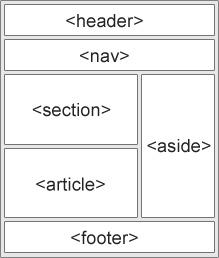
\includegraphics{layout}}
					{\caption{Layout Diagram}}
				\killfloatstyle
				\ttabbox
					{\begin{tabular}{l p{5cm} l}
						\toprule
						Tag & Definition \\\midrule
						\texttt{<header>} & Defines a header for a document or a section \\\midrule
						\texttt{<nav>} & Defines a container for navigation links \\\midrule
						\texttt{<section>} & Defines a section in a document \\\midrule
						\texttt{<aside>} & Defines a sidebar (content aside from the container) \\\midrule
						\texttt{<details>} & Defines additional details \\\midrule
						\texttt{<summary>} & Defines a heading for the details element \\
						\bottomrule
					\end{tabular}}
					{\caption{Tag Definition}}
			\end{floatrow}
		\end{figure}
\end{document}